\documentclass[10pt, 
a4paper, 
oneside, 
headinclude, footinclude, 
BCOR5mm]
{scrartcl}

% Required packages
\usepackage[
    nochapters, beramono, eulermath, pdfspacing, dottedtoc,
]{classicthesis}
\usepackage{arsclassica}
\usepackage[T1]{fontenc}
\usepackage[utf8]{inputenc}
\usepackage{graphicx}
\graphicspath{}
\usepackage{enumitem}
\usepackage{lipsum}
\usepackage{subfig}
\usepackage{amsmath,amssymb,amsthm}
\usepackage{varioref}
\usepackage{titlesec}
\usepackage{color}
\usepackage[linesnumbered, lined, ruled, commentsnumbered]{algorithm2e}

% Adjust title size
\titleformat*{\section}{\color{RoyalBlue}\LARGE}
\titleformat*{\subsection}{\color{black}\Large}
\titleformat*{\subsubsection}{\color{gray}}
\titleformat*{\paragraph}{\large}

% Theorem Styles

% Style used for definitions and examples
\theoremstyle{definition}
\newtheorem*{definition}{Definition}

% Style used for theorems, lemmas, propositions, corollaries
\theoremstyle{plain}
\newtheorem{theorem}{Theorem}[section]
\newtheorem{lemma}{Lemma}

% Style used for remarks and notes
\theoremstyle{remark}

% Set up algorithm 
\SetAlgoLined
\SetKwData{Left}{left}\SetKwData{This}{this}\SetKwData{Up}{up}
\SetKwFunction{Union}{Union}\SetKwData{FindCompress}{FindCompress}
\SetKwInOut{In}{input}\SetKwInOut{Out}{output}
\newcommand\mycommfont[1]{\footnotesize\ttfamily\textcolor{purple}{#1}}

% Hyperlinks
\hypersetup{
colorlinks=true, breaklinks=true, bookmarksnumbered, urlcolor=webbrown, 
linkcolor=RoyalBlue, citecolor=webgreen,
pdfauthor={\textcopyright},
pdfsubject={},
pdfkeywords={},
pdfcreator={pdfLaTeX},
pdfproducer={LaTeX with hyperref and ClassicThesis}
}

\hyphenation{Fortran hy-phen-ation}

%----Title and Authors----%
\title{\normalfont\spacedallcaps{CPSC 331: Data Structures, Algorithms, and their Analysis}}
\author{\spacedlowsmallcaps{Go Uezono}}

\begin{document}

%----Headers----%
\renewcommand{\sectionmark}[1]{\markright{\spacedlowsmallcaps{#1}}}
\lehead{\mbox{\llap{\small\thepage\kern1em\color{halfgray} \vline}\color{halfgray}\hspace{0.5em}\rightmark\hfil}}

\pagestyle{scrheadings}

%----Table of Contents----%
\maketitle
\setcounter{tocdepth}{2}
\tableofcontents
\listoffigures
\listoftables

\newpage
%Algorithmic Analysis%
\section{Algorithmic Analysis}
\subsection{Mathematical Induction}
\subsection{Loop Invariants}
\subsection{Bound Functions}

%-----------------------------------------------------------------------------------%
%Elementary Data Structures%
\section{Elementary Data Structures}

%-----------------------------------------------------------------------------------%
%--Lists--%
\subsection{Lists}

%-----------------------------------------------------------------------------------%
%--Stacks--%
\subsection{Stacks}

%-----------------------------------------------------------------------------------%
%--Queues--%
\subsection{Queues}

%-----------------------------------------------------------------------------------%
%Data Structures%
\section{Data Structures}
%--Binary Search--%
\subsection{Binary Search Trees}

\newpage

%-----------------------------------------------------------------------------------%
%--Red and Black Trees--%
\subsection{Red and Black Trees}
%----Properties----%
\subsubsection{Properties}
A \textbf{red-black tree} is a concrete implementation of a \textbf{self-balancing binary-search tree} (reference here) that automatically maintains balance. 
Giving each node their respective color ensures that no path is more than twice as long as any other, thus is able to maintain approximate balance.\
\begin{enumerate}
    \item Every node is {\color{red}red}/black
    \item Root must be black
    \item Leaves (\textit{null}) are black
    \begin{itemize}
        \item \textit{null} vertices contain no values, while other (interior) do
    \end{itemize}
    \item If a node is {\color{red}red}, then both its children are black
    \item For each node, all simple paths from the node to descendant leaves contain the same number of black nodes 
\end{enumerate}

%----Lemma----%
The following \textbf{lemma} shows why red-black trees make good search trees:
\begin{lemma}
    A red-black tree with $n$ internal nodes has height at most $2\log (n+1)$
\end{lemma}
\begin{proof}
    Start by showing subtree rooted at any ndoe $x$ x contains at least a $2^{bh(x)}-1$ internal nodes. We prove this by \textbf{mathematical induction} on the height of $x$.
    \begin{description}
        \item [\textbf{Claim:}] If height of $x=0$, then the leaf must be \textit{T.null}, and the subtree rooted at $x$ contains at least $2^{bh(x)}-1=2^0-1=0$ internal nodes.
        \begin{description}
            \item [\textbf{Inductive step:}] 
            \begin{itemize}
                \item Consider a node $x$ that has positive height and is an internal node with two children.
                \item Each \textit{child} has a black-height of either $bh(x)$ or $bh(x)-1$ (depending on whether it is {\color{red}red} or black respectively).
                \item Since height of a \textit{child} of $x$ is less than the height of $x$ itself, we can apply the \textbf{I.H} to conlude that:
                \begin{itemize}
                    \item Each child has at least $2^{bh(x)-1}-1$ internal nodes.
                \end{itemize}
            \end{itemize}
            \item Thus, subtree rooted at $x$ contains at least $$(2^{bh(x)-1}-1)+(2^{bh(x)-1}-1)+1$$ internal nodes, which proves the claim.
        \end{description} 
        \item To complete the proof, let $h$ be the height of thr tree. According to property 4 (reference above Properties), at least half the nodes from the root 
        to a leaf (not including the root) must be black.
        \item Consequently, the $bh$ of the root must be at least $h/2$; thus, $$n \geq 2^{h/2}-1$$
        \item Moving $1$ to the left side and taking log on both sides yields: $$\log(n+1) \geq h/2$$ or $$h \leq 2\log(n+1)$$
    \end{description}
\end{proof}

\newpage

%----Rotations----%
\subsubsection{Rotational Properties}
Search operations \textit{TREE-INSERT} and \textit{TREE-DELETE} take $O(\log n)$ time. Since modifications are done to the tree, we must change the color of some of the nodes.
\begin{definition}[\textbf{Rotation}]
    Local operation that preserves the binary-tree property. 
    \begin{itemize}
        \item \textbf{Left Rotation:} assume that its right child $y$ is not \textit{null} 
        \item \textbf{Right Rotation:} assume that its left child $y$ is not \textit{null}
        \begin{itemize}
            \item $x$ can be any node on the tree whose respective child is not \textit{null}
            \item Left/Right rotations "pivots" around the link from $x$ to $y$
            \item Makes $y$ the new root, $x$ as $y$'s left(right) child, $y$'s left(right) child as $x$'s right(left) child
        \end{itemize}
        \item Both L/R rotates run in $O(1)$ time
        \item Only pointers are changed, all attributes in a node remain the same
    \end{itemize}
\end{definition}

\begin{algorithm}
    \caption{Left-Rotate($T,x$)}

    $x = y.right$ \tcp*{set y}
    $x.right = y.left$ \tcp*{Turn y's left subtree into $x$'s right subtree}
    \uIf{$y.left \neq T.null$}
        {$y.left.p = x$\;}
    $y.p = x.p$\;
    \uIf{$x.p == T.null$}
        {$T.root = y$\;}
    \uElseIf{$x == x.p.left$}
        {$x.p.left = y$\;}
    \uElse{$x.p.right = y$\;}
    $y.left = x$\;
    $x.p = y$\;
\end{algorithm}

\newpage 

%----Insertion----%
\subsubsection{Insertion}
Inserting a node can be done in $O(\log n)$ time. Below is a pseudo-code that shows how insertion \textit{RB-INSERT} works:

\begin{algorithm}
    \caption{RB-INSERT$(T,z)$}
    \KwData{$z$ node to insert,}
    \BlankLine

    $y=T.null$\;
    $x=T.root$\;
    \While{$x \neq T.null$}
        {$y=x$\;        
        \eIf{$z.key < x.key$}
            {$x=x.left$\;}
        {$x=x.right$\;}}
    $z.p=y$\;
    \uIf{$y==T.null$}
        {$T.root=z$\;}
    \uElseIf{$z.key < y.key$}
        {$y.left=z$\;}
    \uElse{$y.right=z$\;}
    $z.left=T.null$\;
    $z.right=T.null$\;
    $z.color=T.RED$\;
    RB-INSERT$(T,z)$\;
    
\end{algorithm}

To ensure we preserve the {\color{red}red}-black properties, 
\newpage

%-----------------------------------------------------------------------------------%
%--Heaps--%
\subsection{Heaps}

%----Priority Queues----%
\subsubsection{Priority Queues} \label{subsubsec:prio-q}
\begin{itemize}
    \item Priority queues are \textbf{NOT} FIFO
    \item These queues are interested in removing items (dequeue) with the \textbf{highest priority}
    \item Assume that higher priority value (HPV) entails higher priority
    \begin{itemize}
        \item Not true in general (UNIX OS; smaller PV = higher priority)
    \end{itemize}
    \item Similar operations as the standard Queue ADT:
\end{itemize}

\begin{lstlisting}
    // Queue ADT
    public interface QueueADT<T> {
        public void enqueue(T item);
        public T dequeue(); // different implementation
        public boolean isEmpty();
        public boolean isFull();
    }
\end{lstlisting}
\BlankLine
\paragraph{\textbf{Priority Queue Implementations}}
\begin{itemize}
    \item \textbf{Lists}
    \begin{itemize}
        \item \textbf{Sorted} list by PV with \underbar{array implementation}
        \begin{itemize}
            \item \textit{Ascending order}: Remove \textbf{last} item
            \item \textit{Dequeue}: $O(1)$, \textit{n\textsuperscript{th}} element of the array to be removed
            \item \textit{Enqueue}: $O(n)$, needs to be sorted after enqueue
        \end{itemize}
        \item \textbf{Sorted} list by PV with \underbar{linked-list implementation} 
        \begin{itemize}
            \item \textit{Descending order}: Remove \textbf{first} item
            \item \textit{Ascending order}: Circular list implementation
            \item \textit{Dequeue}: $O(1)$
            \item \textit{Enqueue}: $O(n)$
        \end{itemize}
        \item \textbf{Unsorted} list
        \begin{itemize}
            \item \textit{Dequeue}: $O(n)$
            \item \textit{Enqueue}: $O(1)$
        \end{itemize}
    \end{itemize}
    \item \textbf{BST}
    \begin{itemize}
        \item \textit{Dequeue}: $O(\log(n))$ average-case, $O(n)$ worst-case 
        \item \textit{Enqueue}: $O(\log(n))$ average-case, $O(n)$ worst-case 
    \end{itemize}
    \item \textbf{Heaps}
    \begin{itemize}
        \item \textit{Dequeue}: $O(\log(n))$ worst-case 
        \item \textit{Enqueue}: $O(\log(n))$ worst-case 
    \end{itemize}
\end{itemize}
\newpage

%----Properties----%
\subsubsection{Properties}
A heap is a \textbf{complete} binary tree that satisfies the Heap Property:
\begin{itemize}
    \item Each node of a tree corresponds to an element of an array
    \begin{itemize}
        \item Always stored \textbf{contiguously}
        \begin{itemize}
            \item  If there are blanks, they are on the rightside of the array
            \item  Otherwise, no blanks inbetween indices
        \end{itemize}
    \end{itemize}
    \item It is of height \textit{h} and contains \textit{n} nodes
\end{itemize}

\begin{proof}
    Height \textit{h}
\end{proof}
\BlankLine

\paragraph{\textbf{Heap Properties}} (Figure \vref{fig:heap})
\label{heapproperties}
\begin{itemize}
    \item \textbf{Min Heap Property} 
    \begin{itemize}
        \item Every node has a value $\leq$ than the value of its children
        \item Root of any subtree has the \textit{minimum} value in the subtree    
    \end{itemize}
    \item \textbf{Max Heap Property}
    \begin{itemize}
        \item Every node has a value $\geq$ than the value of its children
        \item Root of any subtree has the \textit{maximum} value in the subtree
    \end{itemize}
    \item \textbf{Child-to-Parent Relation}
    \begin{itemize}
        \item Given a \textbf{child} a location \textit{loc}, what is the index of \textbf{parent} \textit{parent}?
        \item If Child is right, index is \textbf{even}
        \begin{itemize}
            \item $loc_r = 2 \times parent + 2$
        \end{itemize} 
        \item If Child is left, index is \textbf{odd}
        \begin{itemize}
            \item $loc_l = 2 \times parent + 1$
        \end{itemize}
        \item In either cases, $parent = (loc - 1) \div 2$
    \end{itemize}
\end{itemize}
\begin{figure}[H]
    \begin{center}
        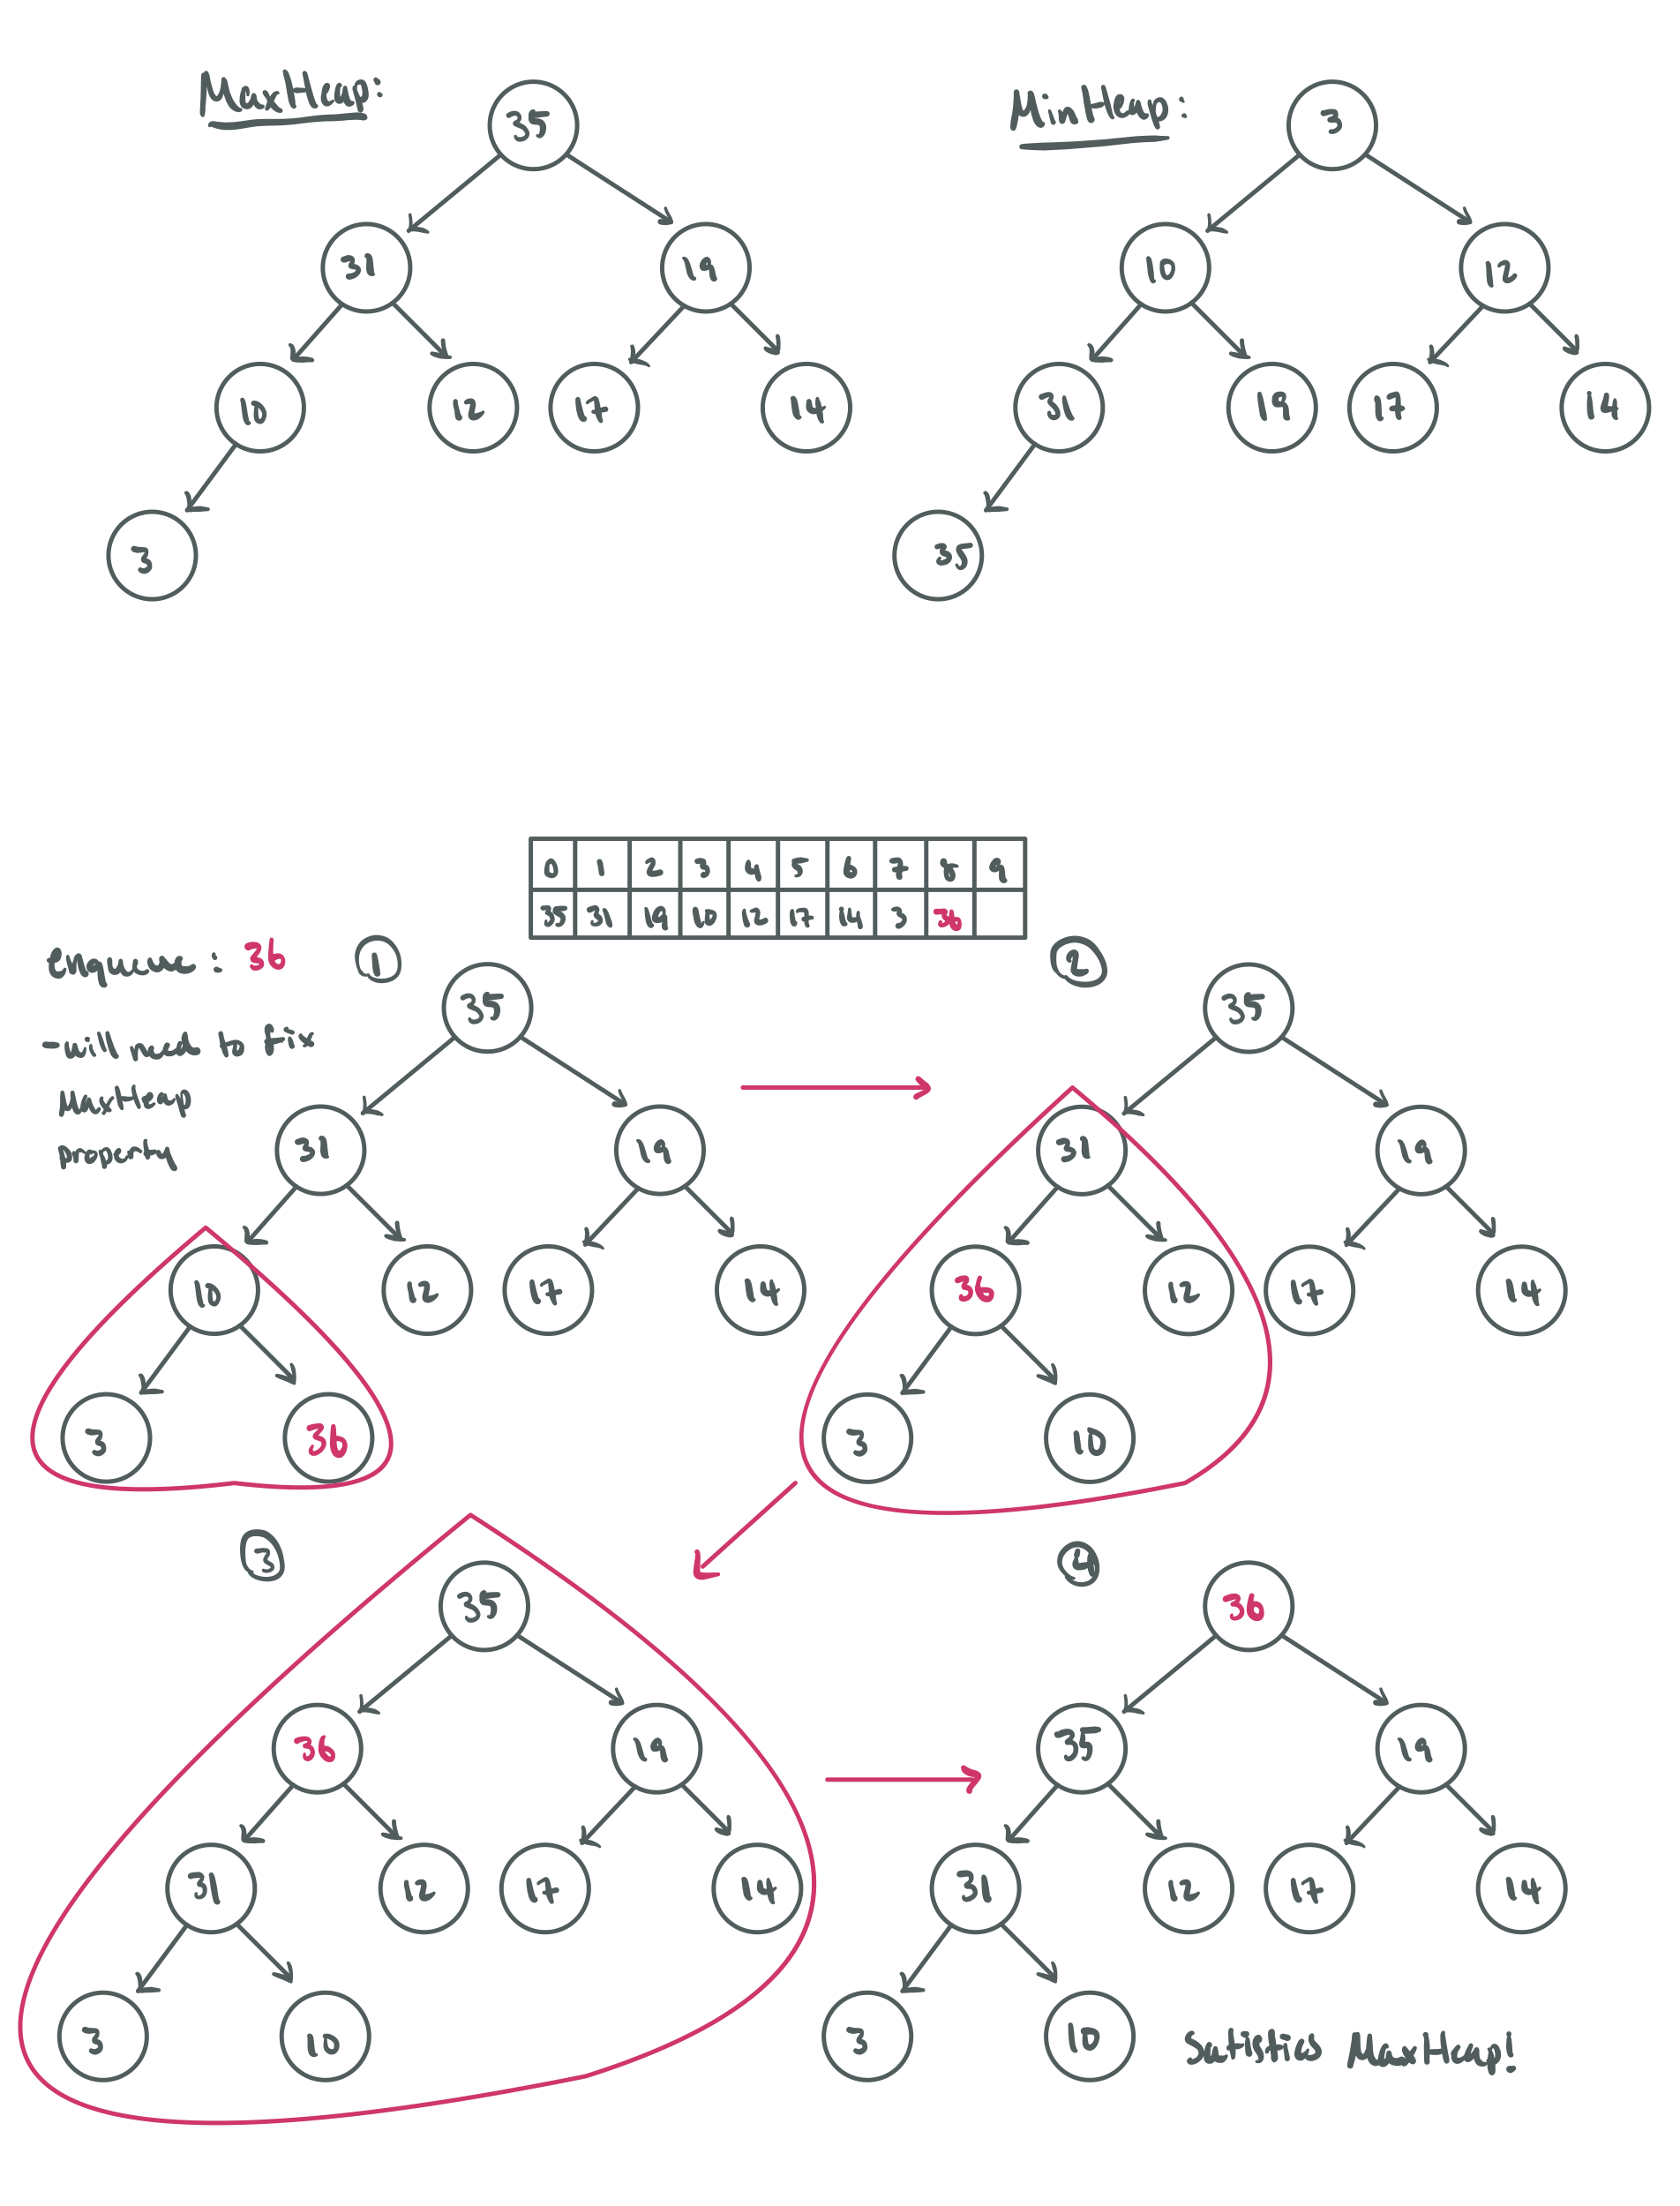
\includegraphics[width=\textwidth]{HeapDiagram.png}
        \caption{MaxHeap/MinHeap Diagram (\vref{heapproperties})}
        \label{fig:heap}
    \end{center}
\end{figure}

%----MaxHeap Class----%
\paragraph{\textbf{MaxHeap Class}}
Similar to the Queue ADT, differences in the enqueue and dequeue functions to maintain \textbf{heap} property
\begin{lstlisting}
    public class MaxHeap<T> {
        private T[] queue;
        private int size;

        public MaxHeap(Class<T> clazz, int maxSize) {
            queue = (T[]) Array.newInstance(clazz, maxSize);
            size = 0;
        }
        public boolean isEmpty() {
            return (size == 0);
        }
        public boolean isFull() {
            return (size == queue.length);
        }
    }
    // enqueue()/dequeue() functions shown later
\end{lstlisting}

%----Enqueue----%
\subsubsection{Insertion}
\begin{definition}
    Inserting an element (Figure \vref{fig:heapenq})
    \begin{itemize}
        \item Must keep the tree \textbf{complete}
        \item Must keep the \textbf{max heap} property
        \item \textbf{Complexity of \textit{Enqueue}}
        \begin{itemize}
            \item \textit{Worst-case}: added node percolates from leaf to root
            \item Since the tree is \textbf{complete}, height is $O(\log(n))$
            \item Hence, \textbf{enqueue} is $O(\log(n))$
        \end{itemize}
    \end{itemize}
\end{definition}
Enqueue:
\begin{lstlisting}
    public void enqueue(T item) {
        queue[size] = item;

        // Fix heap
        int loc = size;
        int parent = (loc - 1)/2;
        while (loc > 0 && queue[loc].compareTo(queue[parent]) > 0) {
            swap(loc, parent);
            loc = parent;
            parent = (loc - 1)/2;
        }
        size++;
    }
\end{lstlisting}
\begin{figure}[H]
    \begin{center}
        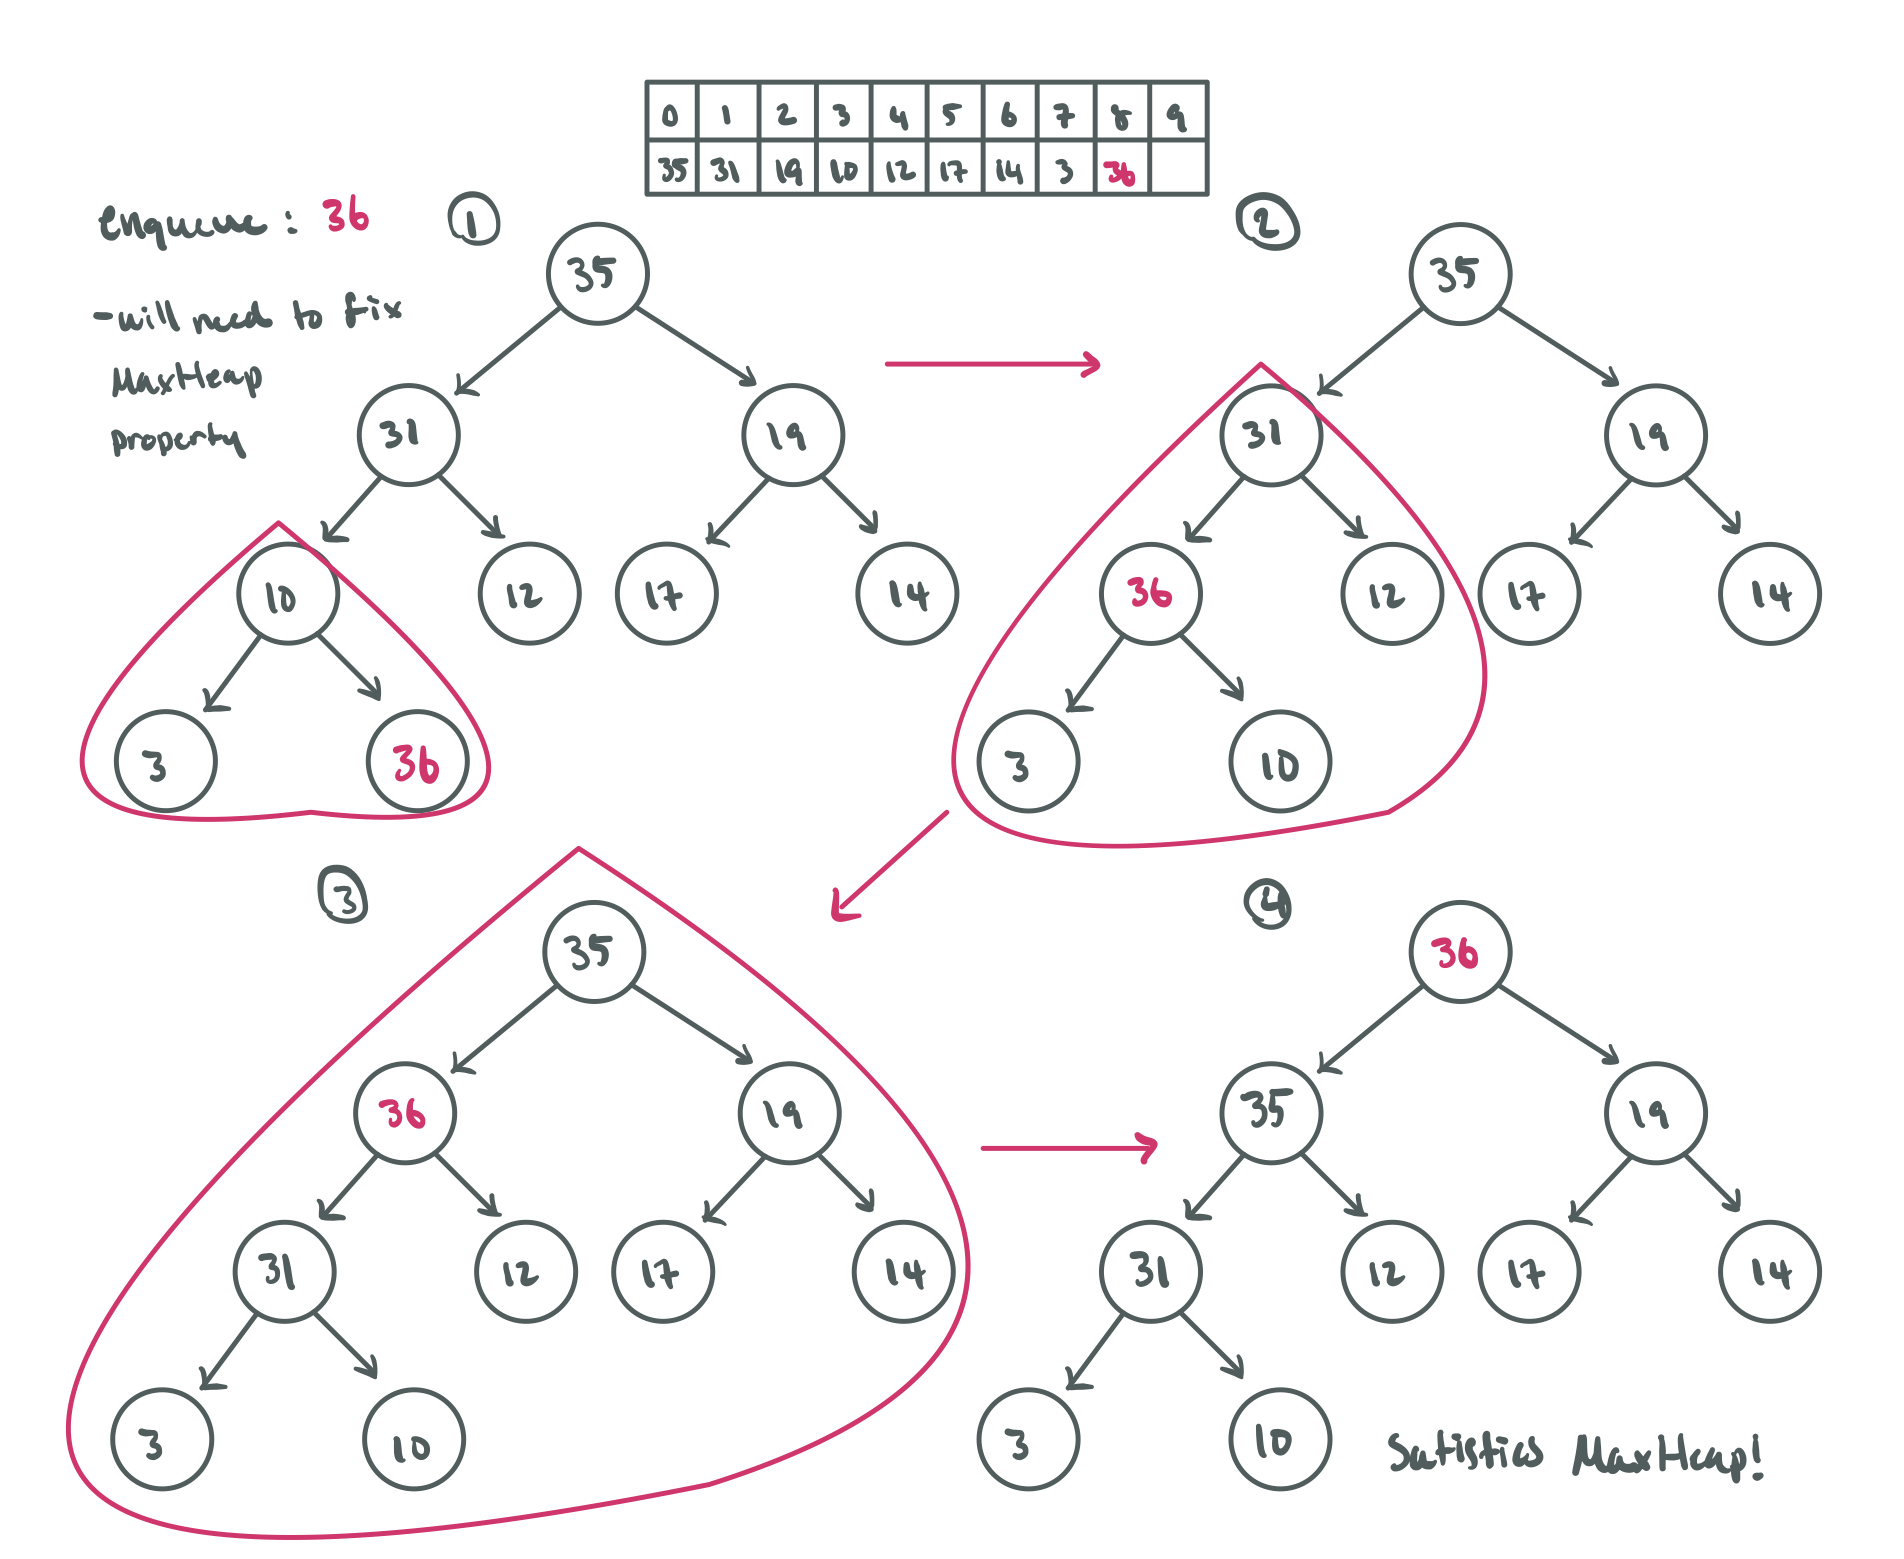
\includegraphics[width=0.9\textwidth]{HeapEnqueue.png}
        \caption{MaxHeap: Enqueue}
        \label{fig:heapenq}
    \end{center}
\end{figure}
Correctness: \textbf{Loop Invariant} for Enqueue
\begin{proof}
        
\end{proof}
\newpage
%----Dequeue----%
\subsubsection{Deletion}
\begin{definition}
    Deleting an element (Figure \vref{fig:heapdeq})
    \begin{itemize}
        \item Must keep the tree \textbf{complete}
        \item Must keep the \textbf{max heap} property 
        \item This process is called \textit{sinking}, where the leaf moves to location (index) 0
        \item We then \textit{sink} the leaf back to its respective location
        \item \textbf{Complexity of \textit{Dequeue}}
        \begin{itemize}
            \item Deleted root "hole" always sinks to a leaf
            \item Since the tree is complete, height is $O(\log(n))$
            \item Hence, \textbf{dequeue} is $O(\log(n))$
        \end{itemize}
    \end{itemize}
\end{definition}
Dequeue
\begin{lstlisting}
    public T dequeue() {
        T max = queue[0];
        queue[0] = queue[size - 1];
        sink(0);
        queue[size - 1] = null;
        size--;
        return max;
     }
\end{lstlisting}
Sink
\begin{lstlisting}
    int swapWith
    int left = 2*loc + 1;
    int right = 2*loc + 2;
    T tmp = queue[loc];

    if (left > (size - 1)) { return;} // Reached a leaf
    else if (left == size - 1) { // Node with one child
        if (tmp.compareTo(queue[left] < 0)) {
            swap(loc, left);
        }
    } else { // Node with two children
        if (queue[left].compareTo(queue[right]) < 0) {
            swapWith = right;
        } else {
            swapWith = left;
        } 
        if (tmp.compareTo(queue[left]) < 0) {
            swap(loc, swapWith);
        }
        sink(swapWith);
    }
\end{lstlisting}
\begin{figure}[H]
    \begin{center}
        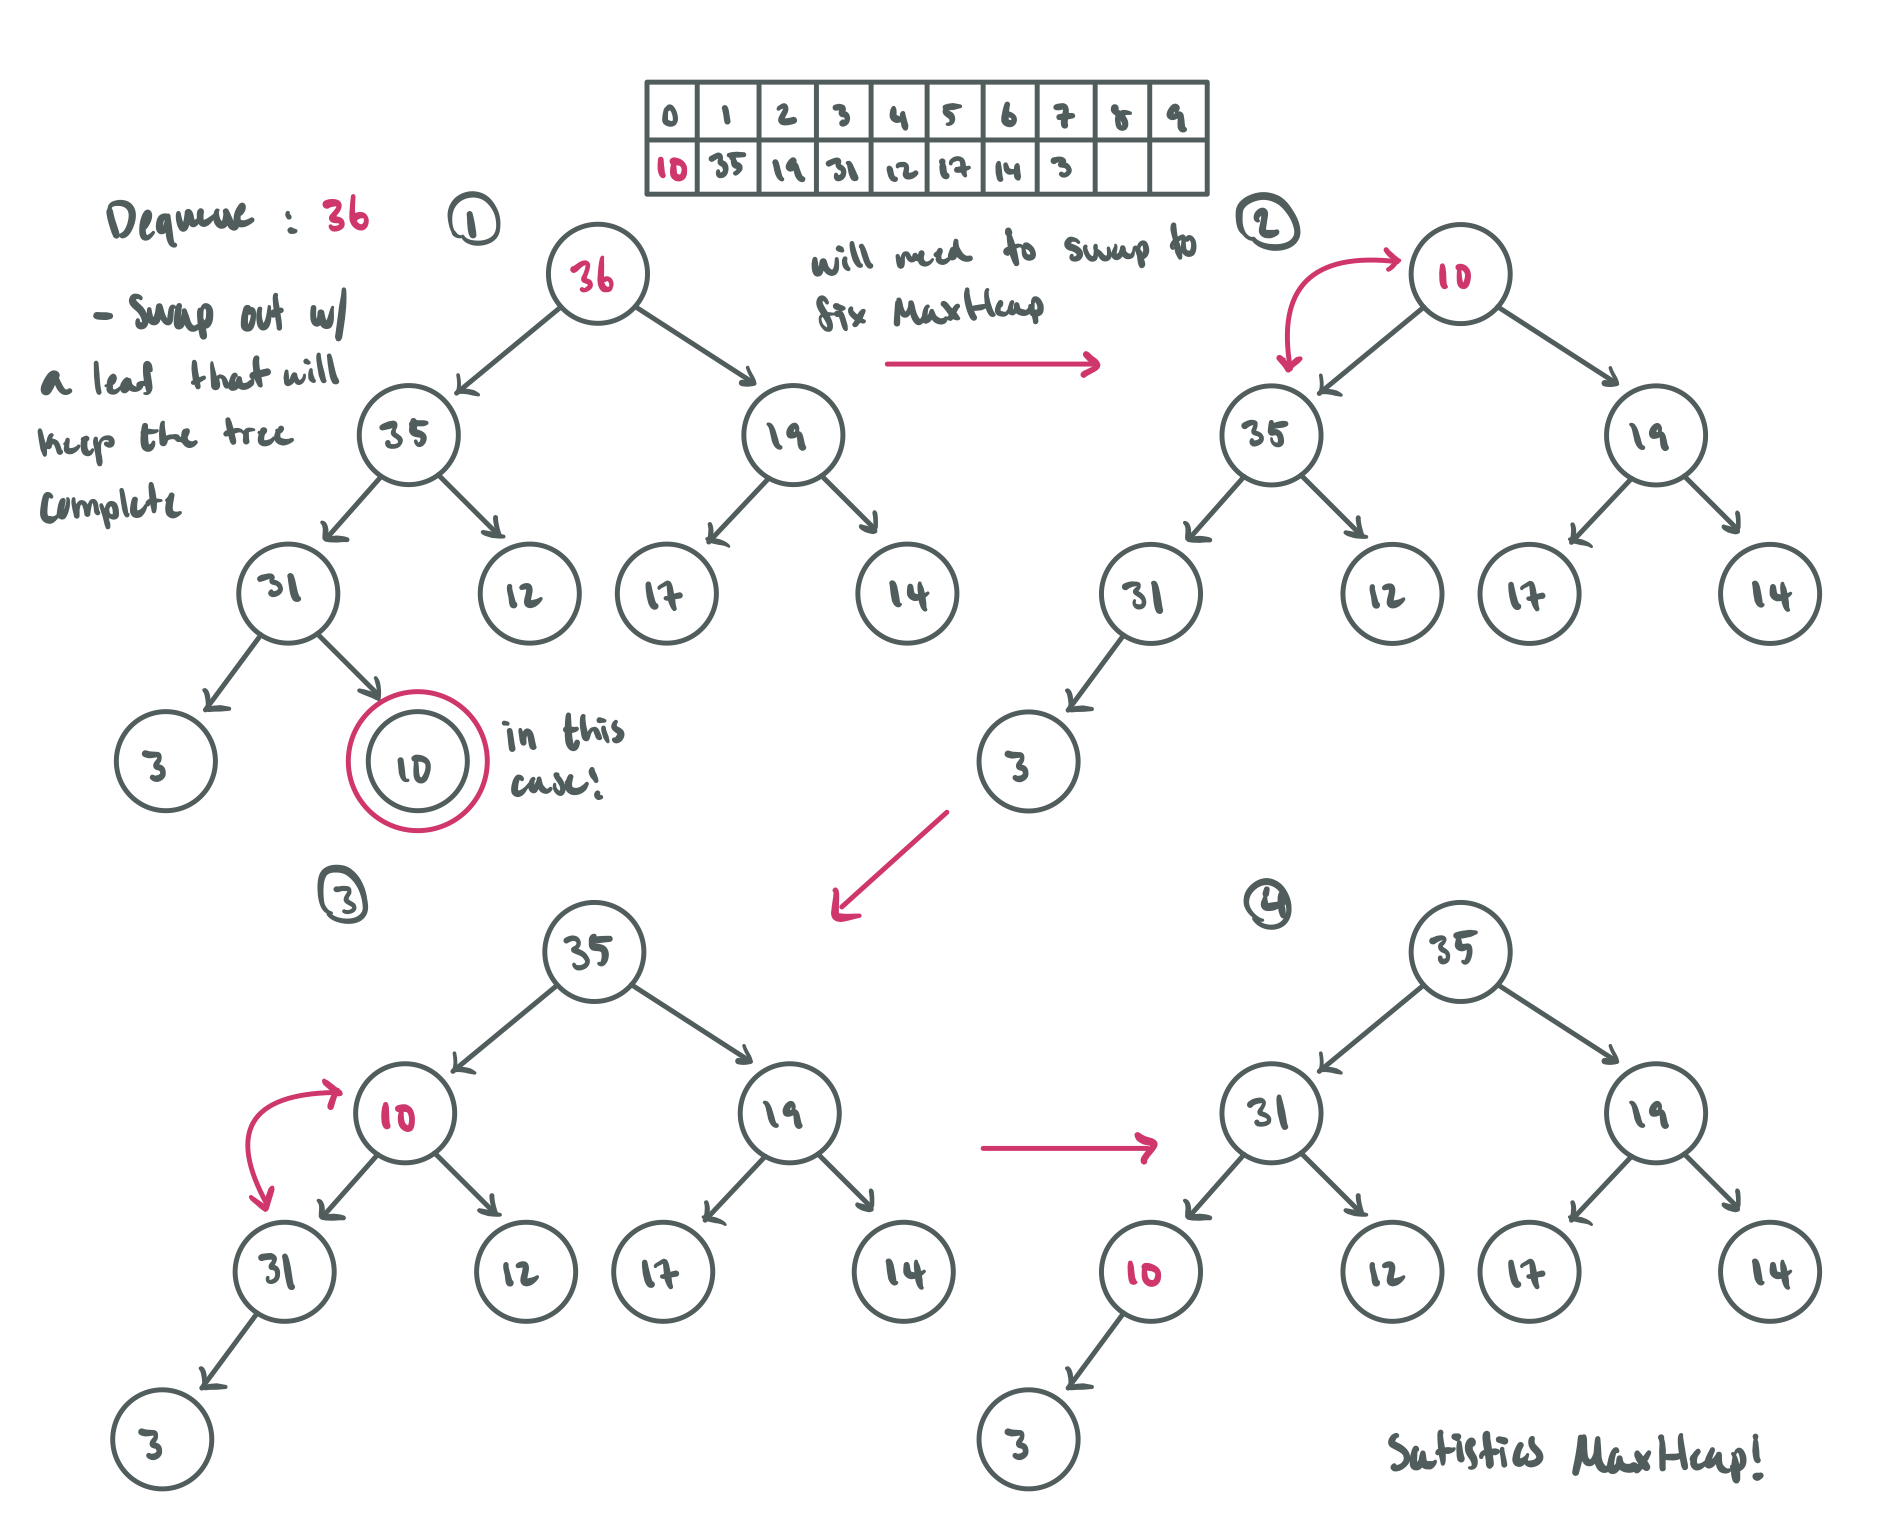
\includegraphics[width=\textwidth]{HeapDequeue.png}
        \caption{MaxHeap: Dequeue}
        \label{fig:heapdeq}
    \end{center}
\end{figure}
Correctness: \textbf{Bound Function} for Dequeue
\begin{proof}
    Prove that sink() maintains heap property
\end{proof}

\newpage
%-----------------------------------------------------------------------------------%
%--Hash Table--%
\subsection{Hash Table}
%----Properties----%
\subsubsection{Properties}
\begin{definition}
    \textit{Hash Table ADT}
    \begin{itemize}
        \item Allows adding, removing, searching for items in $O(1)$ on average
        \item Implementation is called \textit{hashing}
        \item Objects are mapped to a hash table based on a value calculated by a \textbf{hash function}
        using an object's key
        \begin{itemize}
            \item e.g. ID of a Student object as a \textit{key}
        \end{itemize}
        \item Hash function: $$h(x): U \rightarrow \{0, 1, ..., m-1\}$$
        \begin{itemize}
            \item $U\rightarrow$ set of all Objects
            \item $|U| = n$
            \item $m\rightarrow$ hash table size (buckets)
            \item Typically $n>m$ (much larger)
            \item Given an object $x\in U,h(x)$ maps $x$ to a bucket in the hash table
        \end{itemize}
        \item Performance of the hash table is dependent on the quality of the hash function
        \item A \textbf{Good} hash function distributes items \textit{evenly} among buckets in the hash table
    \end{itemize}
\end{definition}
\begin{figure}[H]
    \begin{center}
        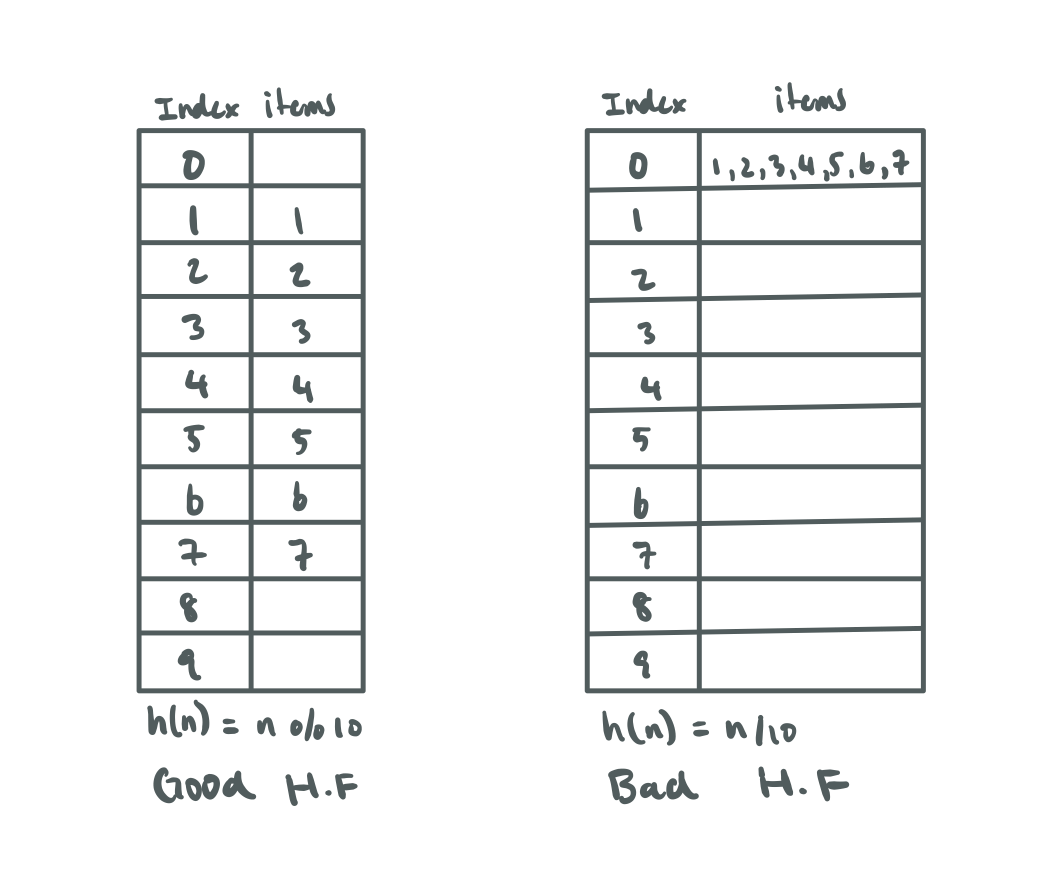
\includegraphics[width=0.95\textwidth]{HashFunction.png}
        \caption{Good vs Bad Hash Functions}
        \label{fig:hashfunc}
    \end{center}
\end{figure}
\textbf{Collisions}
\begin{itemize}
    \item Occurs when two objects map to the same hash value
    \begin{itemize}
        \item Objects $o_1$ and $o_2\rightarrow h(o_1)=h(o_2)$
        \item Unavoidable since $n>m$
    \end{itemize}
    \item Can be dealt with:
    \begin{itemize}
        \item Chaining
        \item Probing/Open addressing
        \item Double hashing
    \end{itemize}
\end{itemize}

%----Chaining----%
\subsubsection{Chaining}
\begin{definition}
    \textit{Chaining}
    \begin{itemize}
        \item Group items with the same hash value (via a hash function) into a bucket (AKA a chain)
        \item e.g. Figure \vref{fig:hashfunc}
        \item \textbf{Time Complexity}:
        \begin{itemize}
            \item \textit{Worst-case}: Hash table becomes a single LL if elements are mapped to one bucket - $O(n)$ search
            \item \textit{Best-case}: Search can become $O(1)$, but is actually $O(n/m)$
            \begin{itemize}
                \item $m$ size of the table, $n$ number of elements to be hashed
            \end{itemize}
        \end{itemize}
    \end{itemize}
\end{definition}

\textbf{Hashable Objects}
\begin{lstlisting}
    public class HashableObject implements Hashable {
        private String key;
        // Other aspects of the object
        public HashableObject(String s) {
            key = new String(s);
        }
        public String key() {
            return key;
        }
    }
\end{lstlisting}

\textbf{3 Hash Functions, each used for different scenarios}
\begin{itemize}
    \item \textit{Hash Function 1}
    \item Fast, but not good for large table sizes
    \begin{lstlisting}
        public class HF1 extends HF {
            public int hash(String s, int size) {
                int hashVal = 0;
                for (int i = 0; i < s.length; i++) {
                    hashVal += s.charAt(i);
                    // Returns int code, e.g. A 65, B 66, etc
                }
                return hashVal % size;
            }
        }
    \end{lstlisting}
    \newpage

    \item \textit{Hash Function 2}
    \item Fast, generally better than HF1, but horrible distributions of values where the first 3 chars are frequent
    \begin{lstlisting}
        public class HF2 extends HF {
            public int hash(String s, int size) {
                int hashVal = 0;
                for (int i = 0; i < s.length; i++) {
                    if (i == 0) { hashVal += s.charAt(0);}
                    else if (i == 1) {hashVal += 27 * s.charAt(1);}
                    else if (i == 2) {hashVal += 729 & s.charAt(2);}
                }
                return hashVal % size;
            }
        }
    \end{lstlisting}

    \item \textit{Hash Function 3}
    \item Fast and has good distribution
    \begin{lstlisting}
        public class HF3 extends HF {
            public int hash(String s, int size) {
                int hashVal = 0;
                for (int i = 0; i < s.length; i++) {
                    hashVal += 37 * hashVal + s.charAt(i);
                }
            hashVal % size;
            if (hashVal < 0) {hashVal += size;}
            return hashVal;
            }
        }
    \end{lstlisting}
\end{itemize}

%----Hash Table implementation with Chaining----%
\textbf{Hash Table implementation with Chaining}
\begin{itemize}
    \item The interface includes clear(), add(), remove(), and contain()
    \begin{lstlisting}
        public class HashTableSC<T extends Hashable> implements HashTableInterface<T> {
            private LinkedList<T>[] hashTable;
            private HashFunction f;

            public HashTableSC(HashFunction f, int m) {
                hashTable = new LinkedList[m];
                this.f = f;
            }
            // Clear 
            public void clear() {
                for (int i = 0; i < hashTable.length; i++) {
                    hashTable[i] = null;
                }
            }
            // Insertion 
            public void add(T item) {
                int i = f.hash(item.key(), hashTable.length);
                if (hashTable[i] == null) {
                    hashTable[i] = new LinkedList<T>();
                }
                hashTable[i].add(item);
            }

            // Deletion
            public void remove(T item) {
                hashTable[f.hash(item.key(), hashTable.length)].remove(item.key());
                // Code before .remove will give you the Chain
            }
            // Search
            public boolean contains(T item) {
                int i = f.hash(item.key(), hashTable.length);
                if (hashTable[i] == null) {return false; }
                else {return hashTable[i].contains(item); }
            }
        }
    \end{lstlisting}
    \item \textbf{Correctness}: follows the correctness of regular LL operations
    \item \textbf{Time Complexity} (with Chaining):
    \begin{itemize}
        \item \textit{Load factor} $\lambda$ of a hash table is the average length of chains $$(n_0+n_1+...+n_{m-1})/m = n/m = \lambda$$
        \item Search analysis: $O(1+\lambda)$, but can be proven $\theta(1+\lambda)$ 
        \item Insertion analysis: \textbf{Average}: $\theta(1)$, \textbf{W.C}: $O(n)$
        \item Deletion analysis: \textbf{Average}: $O(1+\lambda)$, \textbf{W.C}: $O(n)$
    \end{itemize}
\end{itemize}

%----Open Addressing----%
\subsubsection{Open Addressing}
\begin{definition}
    \textbf{Open Addressing}
    \begin{itemize}
        \item Method for handling collisions
        \item All elements are stored in the hash table
        \item When \textit{collision} occurs, probe the table until a free (null) entry is found
        \begin{figure}[H]
            \begin{center}
                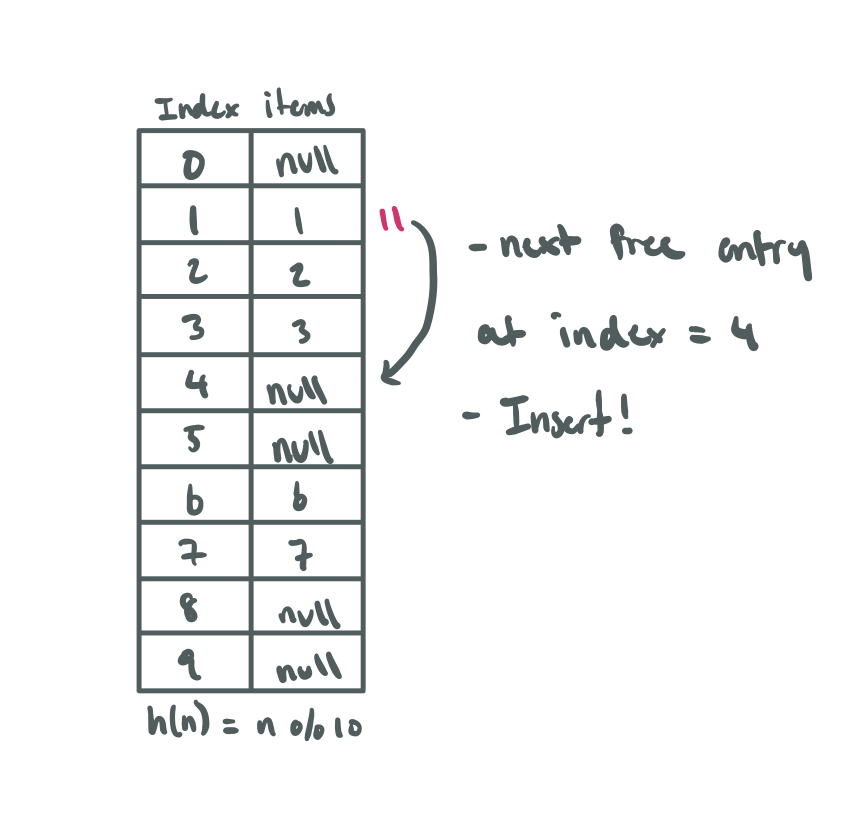
\includegraphics[width=0.6\textwidth]{OpenAddressing.png}
                \caption{Insert 11 in hash table (via hash function)}
            \end{center}
        \end{figure}
        \item \textbf{Linear Probing}
        \begin{itemize}
            \item Prior to inserting 11 at index 4, we had to go through previous indicies to check if they were free
            \item That is $\rightarrow h(k)+0, h(k)+1, h(k)+2, h(k)+3$
            \item Can be represented by: $<h(k),0>,<h(k),1>,<h(k),2>,...$
            \item This is the \textbf{probing sequence}, which gives us a new hashing function $$h'(k)=h(k)+(i \mod 10)$$
            \item This is called \textbf{Linear Probing}
            \begin{itemize}
                \item Variations: Quadratic, double-hashing, etc.
            \end{itemize} 
        \end{itemize}
    \end{itemize}
\end{definition}

%----Algorithms for Linear Probing----%
\textbf{Algorithms for Linear Probing}
\begin{algorithm}
    \caption{Inserting a key \textit{k}}
    $i = 0$\;
    \While{$i<m$}
        {$j=h(k,i)$\;
        \uIf{($T[j]==null$ or $T[j]==Deleted$)}
            {$T[j]=k$\;
            return j\;}
        $i=i+1$\;}
    Throw a TableFullException\;
\end{algorithm}
\textbf{Example of Insertion}
\begin{figure}[H]
    \begin{center}
        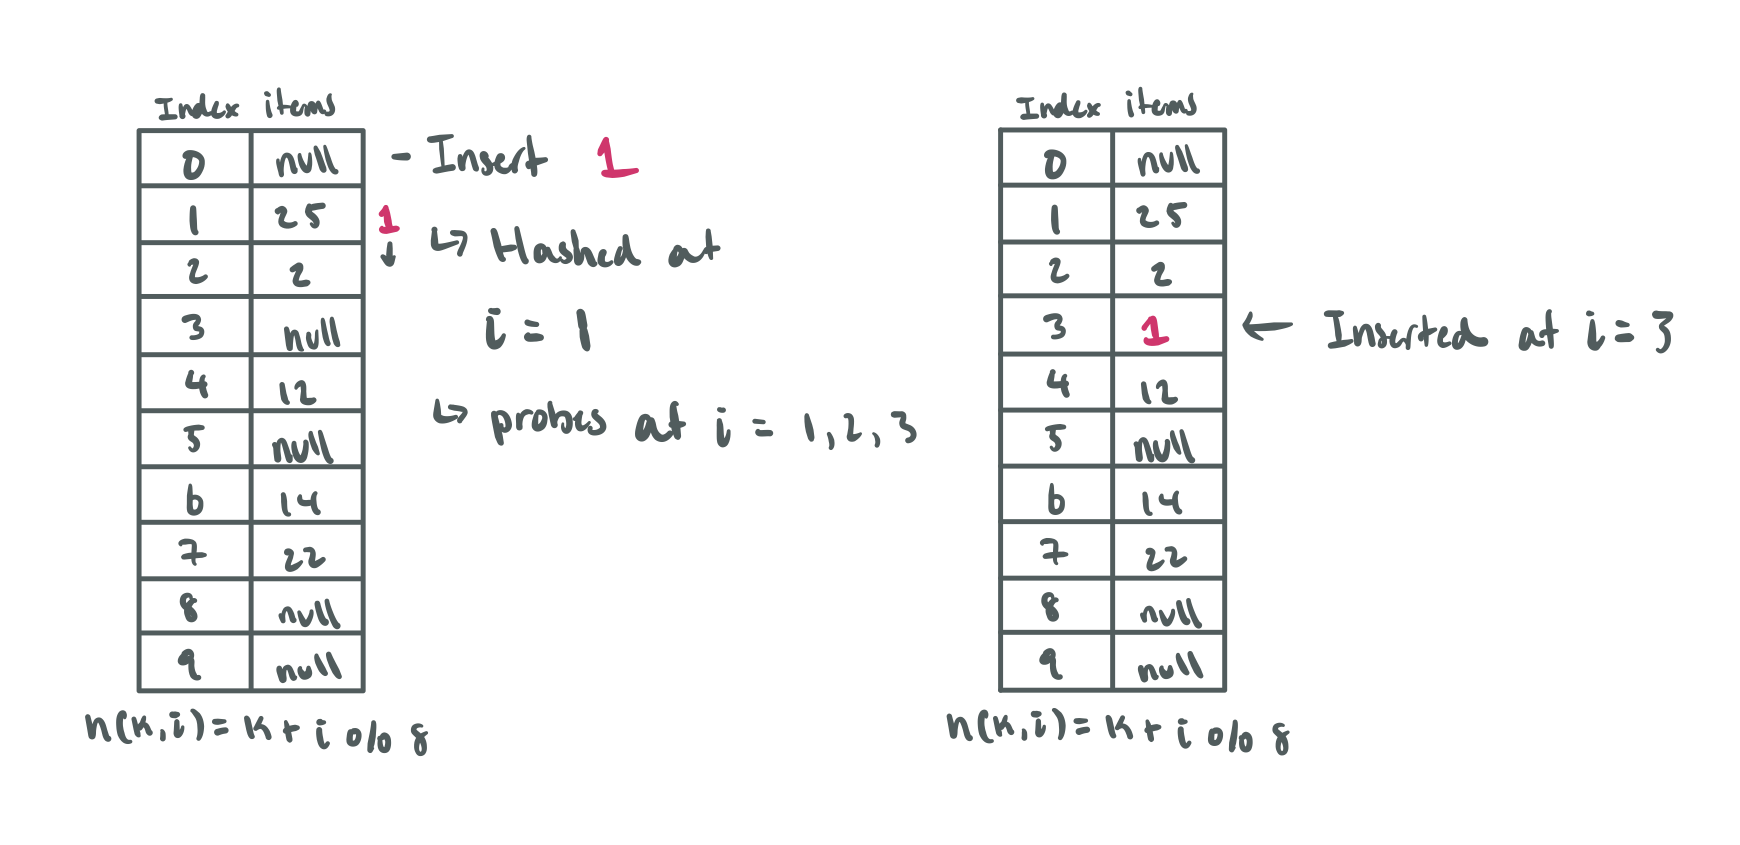
\includegraphics[width=\textwidth]{OAInsert.png}
        \caption{Insert 1}
    \end{center}   
\end{figure}

\begin{algorithm}
    \caption{Searching a key \textit{k}}
    $i = 0$\;
    \While{$i<m$}
        {$j=h(k,i)$\;
        \uIf{($T[j]==k$)}
            {return j\;}
        \uElseIf{$T[j]==null$}
            {Throw a NoSuchElementException\;}
        $i=i+1$\;}
\end{algorithm}
\newpage
\textbf{Example of Searching}
\begin{figure}[H]
    \begin{center}
        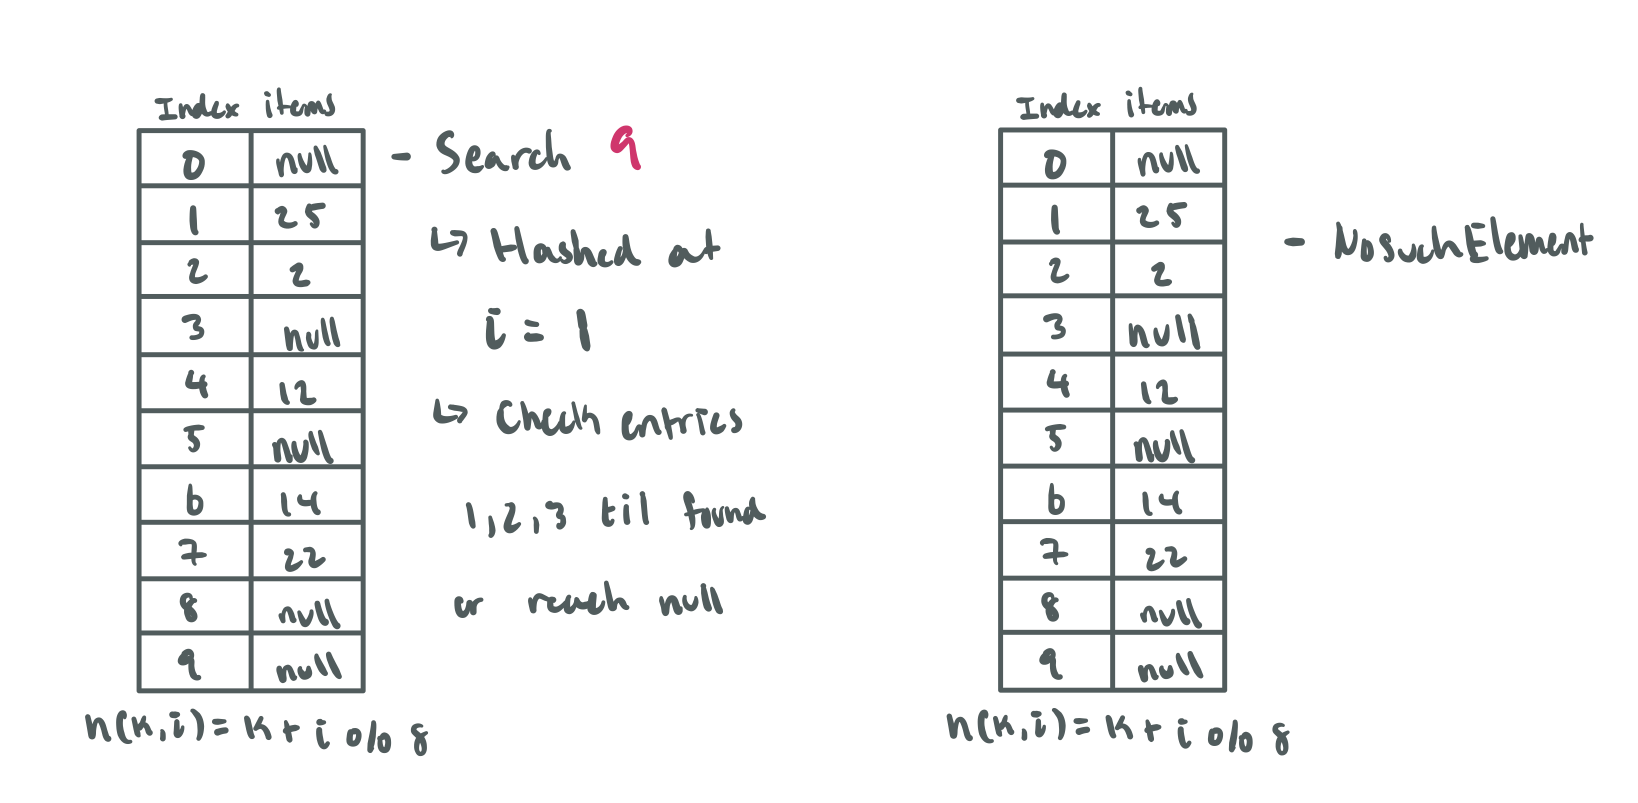
\includegraphics[width=\textwidth]{OASearch.png}
        \caption{Search 9}
    \end{center}   
\end{figure}

\begin{algorithm}
    \caption{Deleting a key \textit{k}}
    $i = 0$\;
    \While{$i<m$}
        {$j=h(k,i)$\;
        \uIf{($T[j]==k$)}
            {$T[j]==deleted$\;
            return\;}
        \uElseIf{($T[j]==null$)}
            {Throw a NoSuchElementException\;}
        $i=i+1$\;}
    Throw a NoSuchElementException\;
\end{algorithm}
\newpage
\textbf{Example of Deletion}
\begin{figure}[H]
    \begin{center}
        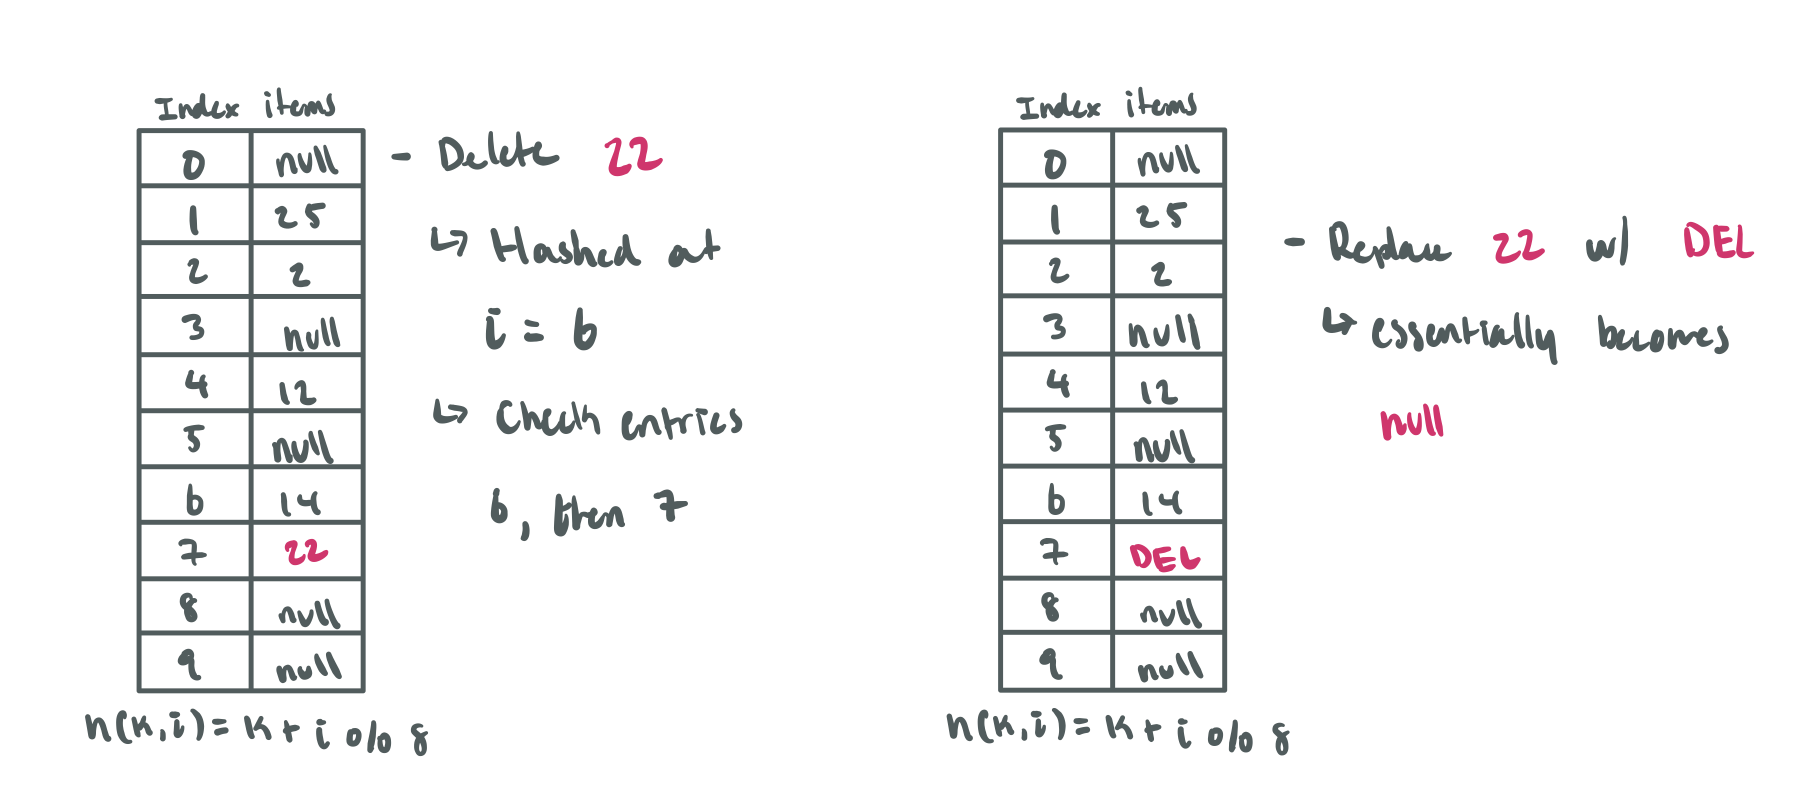
\includegraphics[width=\textwidth]{OADelete.png}
        \caption{Delete 22}
    \end{center}   
\end{figure}

\newpage
%-----------------------------------------------------------------------------------%
%--Graphs--%
\subsection{Graphs}

\newpage
%-----------------------------------------------------------------------------------%
%--Dijkstra's Algorithm--%
\subsection{Dijkstra's Algorithm}

\newpage
%-----------------------------------------------------------------------------------%

%Sorting Algorithms%
\section{Sorting Algorithms}
%--Bubble Sort--%
\subsection{Bubble Sort}
%----Algorithm----%
\subsubsection{Bubble Sort Algorithm}
\begin{lstlisting}
    // Bubble Sort in Sorting
    public void sort() {
        for (i = 0; i < size; i++) {
            for (j = size - 1; j > i; j--) {
                if (list[j].compareTo(list[j-1]) < 0) {
                    T tmp = list[j];
                    list[j] = list[j-1];
                    list[j-1] = tmp;
                }
            }
        }
    }
    // Bubble Sort in BoundedList
    public static void sort(BoundedList list) {
        for (i = 0; i < list.size(); i++) {
            for (j = list.size() - 1; j > i; j--) {
                if (list.getItem(j).compareTo(list.getItem(j-1)) < 0) {
                    list.swap(j, j-1);
                }
            }
        }
    }
    // Main algorithm
    Bubble-Sort(L = list of items, n = size) {
        for (i = 0; i < n; i++) {
            for (j = n - 1; j > i; j--) {
                if (L[j].key < L[j-1].key) {
                    swap(L[j], L[j-1]);
                }
            }
        }
    }
    // Where swap() is...
    swap(item n1, item n2) {
        tmp = n1;
        n1 = n2;
        n2 = tmp;
    }
\end{lstlisting}
\newpage
\textbf{Example}:
\begin{figure}[H]
    \begin{center}
        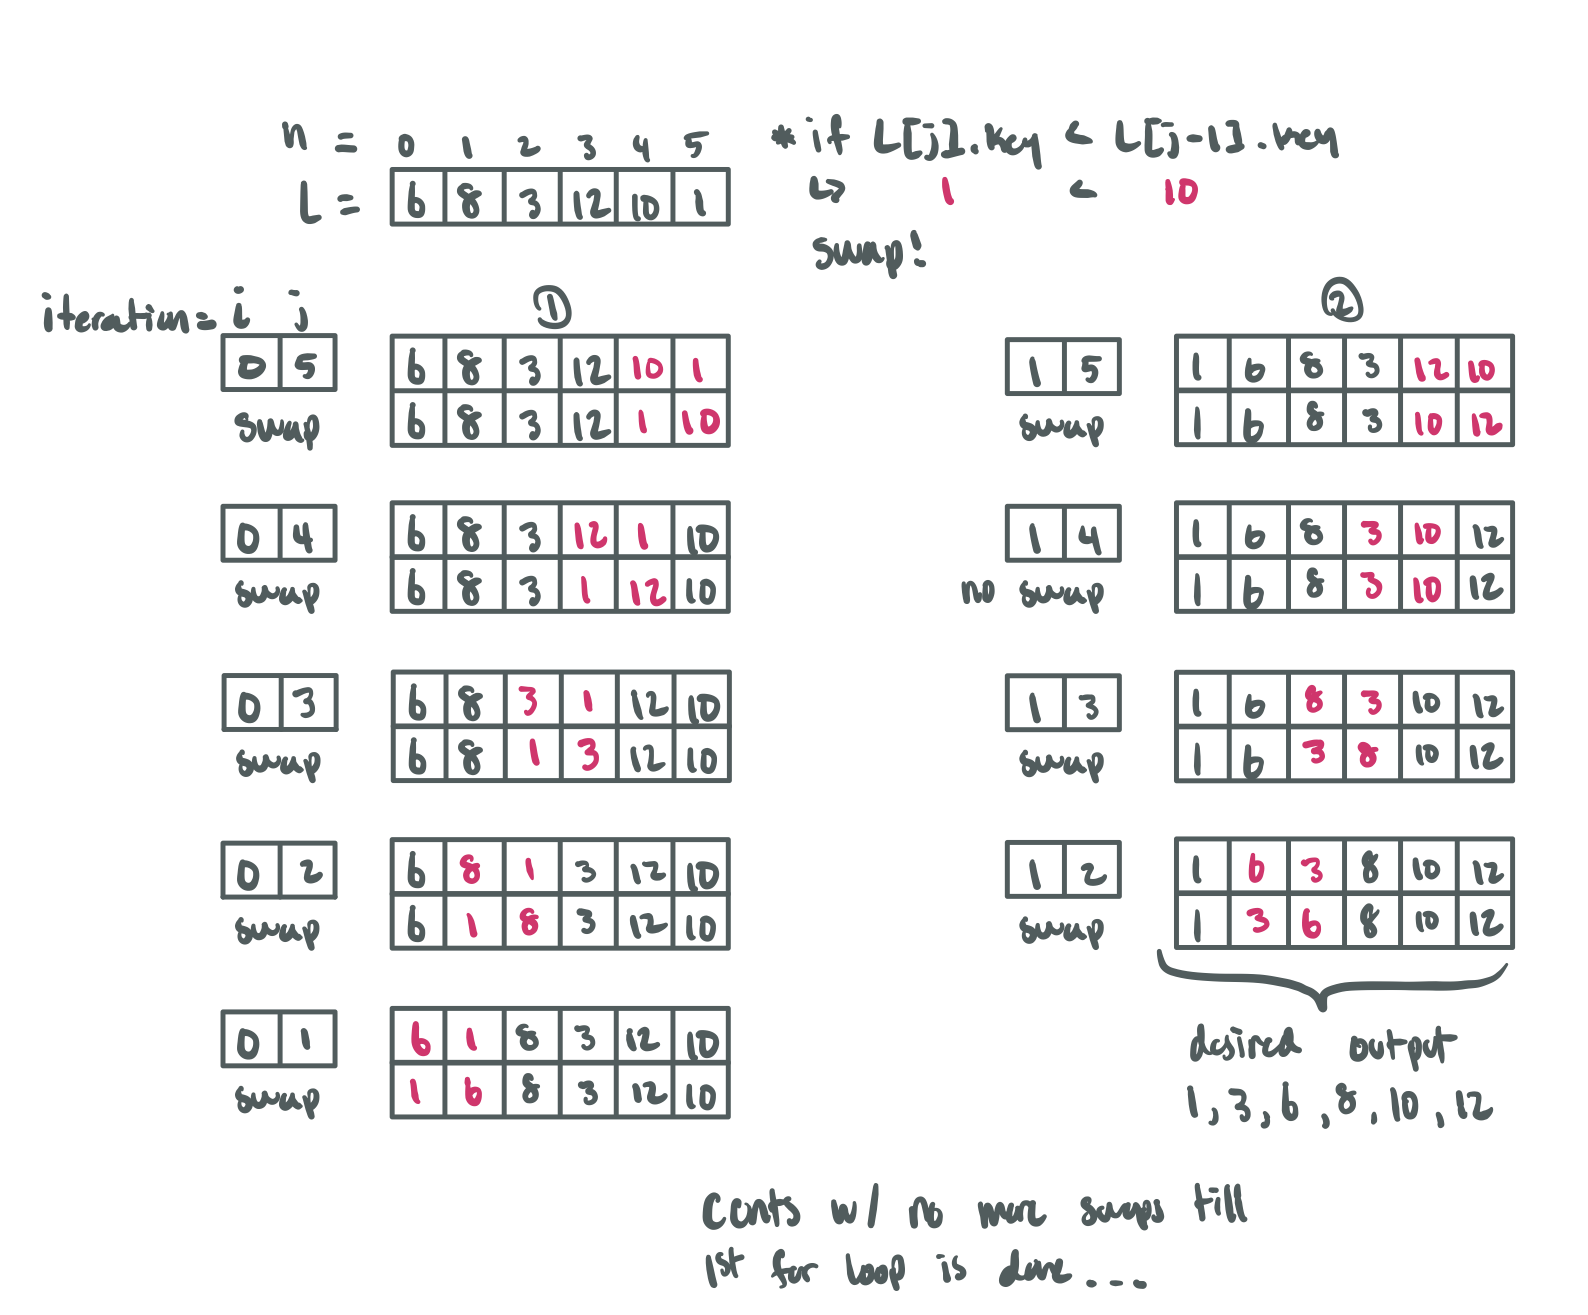
\includegraphics[width=\textwidth]{BubbleSort.png}
        \caption{Bubble sort following the main algorithm}
    \end{center}
\end{figure}

%----Time Complexity----%
\subsubsection{Time Complexity}
\begin{definition}
    \textit{Time Complexity}
    \begin{itemize}
        \item \textbf{swap()}: $\theta(1)$
        \item \textbf{j-loop}: executed $n-i-1$ times
        \item \textbf{i-loop}: executed $n$ times
        \item \textbf{Bubble-Sort}: $\Sigma^{n-1}_{i=0}n-i-1$ $$\Sigma^{n-1}_{i=0}n-i-1=(n-1)+(n-2)+...+1+0=\frac{n^2-n}{2}$$
        \item \textbf{Hence}, Bubble-Sort is quadratic, $\theta(n^2)$
    \end{itemize}
\end{definition}
\newpage

%----Correctness----%
\subsubsection{Correctness}
\begin{definition}
    \textit{Loop Invariant}
    \begin{itemize}
        \item \textbf{Inner Loop}
        \begin{itemize}
            \item \textit{Initialization}:
            \begin{itemize}
                \item Initially, $j=n-1$ and $L[n-1...n-1]$ is a singleton
                \begin{itemize}
                    \item LI is vacuously satsified
                \end{itemize}
            \end{itemize}
            \item \textit{Maintenance}:
            \begin{itemize}
                \item Assume LI is correct before iteration $j=k$
                \item That is, $L[k]$ is the min in $L[k...n-1]$
                \item In iteration $j=k$
                \begin{itemize}
                    \item If $L[k].key<L[k-1].key$, then swap($L[k],L[k-1]$), making $L[k-1]$ the new min in $L[k-1...n-1]$
                    \item Else, item being considered $L[k-1]$ is not bigger than $L[k]$, meaning that $L[k-1]$ is the min in $L[k-1...n-1]$
                    \item Hence, before the next iteration $j=k-1$, $L[k-1]$ is the min in $L[k-1...n-1]$
                \end{itemize}
            \end{itemize}
            \item \textit{Termination}:
            \begin{itemize}
                \item Last iteration of the loop is when $j=i-1$
                \item Hence, by LI, $L[i]$ is the min item in $L[i...n-1]$
            \end{itemize}
        \end{itemize}
        \item \textbf{Outer Loop}
        \begin{itemize}
            \item \textit{Initialization}:
            \begin{itemize}
                \item Before the first iteration, $i=0$ and $L[0...i-1]$ is empty and LI is vacuously true
            \end{itemize}
            \item \textit{Maintenance}:
            \begin{itemize}
                \item Assume LI is correct before iteration $i=k$
                \item Hence, $L[0...k-1]$ is a sorted list of the smallest \textit{k} items in L
                \item In iteration $i=k$, by the LI of the \textbf{inner loop}:
                \begin{itemize}
                    \item $L[k]$ is the min item in $L[k...n-1]$
                \end{itemize}
                \item Since $L[0...k-1]$ has the smallest \textit{k} items of L in sorted order,
                \item $L[0...k]$ will have the smallest $k+1$ items in L in sorted order
            \end{itemize}
            \item \textit{Termination}:
            \begin{itemize}
                \item Last iteration of the loop is when $i=n-1$
                \item Hence, when the loop terminates, $L[0...n-2]$ is a sorted permutation of the smallest $n-1$ elements in L
                \item Since $L[n-1]$ was considered the last iteration and compared with $L[n-2]$, it must be the case that $L[n-1]$ is the largest 
                item in L
                \item Therefore, when the loop terminates, $L[0...n-1]$ is a sorted permutation of the original elements in L
            \end{itemize}
        \end{itemize}
    \end{itemize}
\end{definition}
\newpage
%-----------------------------------------------------------------------------------%
%--Selection Sort--%
\subsection{Selection Sort}
%----Algorithm----%
\begin{lstlisting}
    // Selection sort in Sorting
    public static void selectionSort(BoundedList list) {
        for (int i = 0; i < list.size(); i++) {
            int minIndex = list.getMinIndex(i, list.size()-1);
            list.swap(i, minIndex);
        }
    }
    // Main algorithm
    Selection-Sort(L = list of items, n = size) {
        for (i = 0; i < n; i++) {
            min = Find-Min(L[i...n-1]);
            swap(L[i], min);
        }
    }
    // Find minimum
    Find-Min(L = list of items, n = size) { // Must be non-empty
        currMin = L[0];
        for (i = 1; i < n; i++) {
            if (L[i] < currMin) {
                currMin = L[i];
            }
        }
        return currMin;
    }
\end{lstlisting}
\textbf{Example}:
\begin{figure}
    \begin{center}
        %\includegraphics[options]{name}
        \caption{Selection sort following main algorithm}
    \end{center}
\end{figure}

%----Time Complexity----%
\begin{definition}
    \textit{Time Complexity}
    \begin{itemize}
        \item \textbf{loop}: executed $n-1$ times
        \item \textbf{Find-Min()}: $\theta(n)$ on all cases
        \begin{itemize}
            \item List is reduced by 1 after every iteration
            \item 1st: $|L|=n$
            \item 2nd: $|L|=n-1$
            \item ith: $|L|=n-i-1$
        \end{itemize}
        \item \textbf{Selection-Sort}: $\Sigma^{n-1}_{i=1}n-i-1$ $$\Sigma^{n-1}_{i=1}n-i-1=(n-2)+...+1=\frac{n^2-2n+2}{2}$$
        \item \textbf{Hence}, Selection-Sort is quadratic, $\theta(n^2)$
    \end{itemize}
\end{definition}
%----Correctness----%
\newpage
%-----------------------------------------------------------------------------------%
%--Insertion Sort--%
\subsection{Insertion Sort}
%----Algorithm----%
\begin{lstlisting}
    // Insertion Sort in Sorting
    public static void sort(BoundedList list) {
        for (i = 1; i < list.size(); i++) {
            for (j = i; j > 0; j--) {
                if (list.getItem(j).compareTo(list.getItem(j-1)) < 0) {
                    list.swap(j, j-1);
                }
            }
        }
    }
    // Main algorithm
    Insertion-Sort(L = list of items, n = size) {
        for (i = 1; i < n; i++) {
            for (j = i; j > 0; j--) {
                if (L[j].key < L[j-1].key) {
                    swap(L[j], L[j-1]);
                }
            }
        }
    }
    // Where swap() is...
    swap(item n1, item n2) {
        tmp = n1;
        n1 = n2;
        n2 = tmp;
    }
\end{lstlisting}
\textbf{Example}:
\begin{figure}[H]
    \begin{center}
        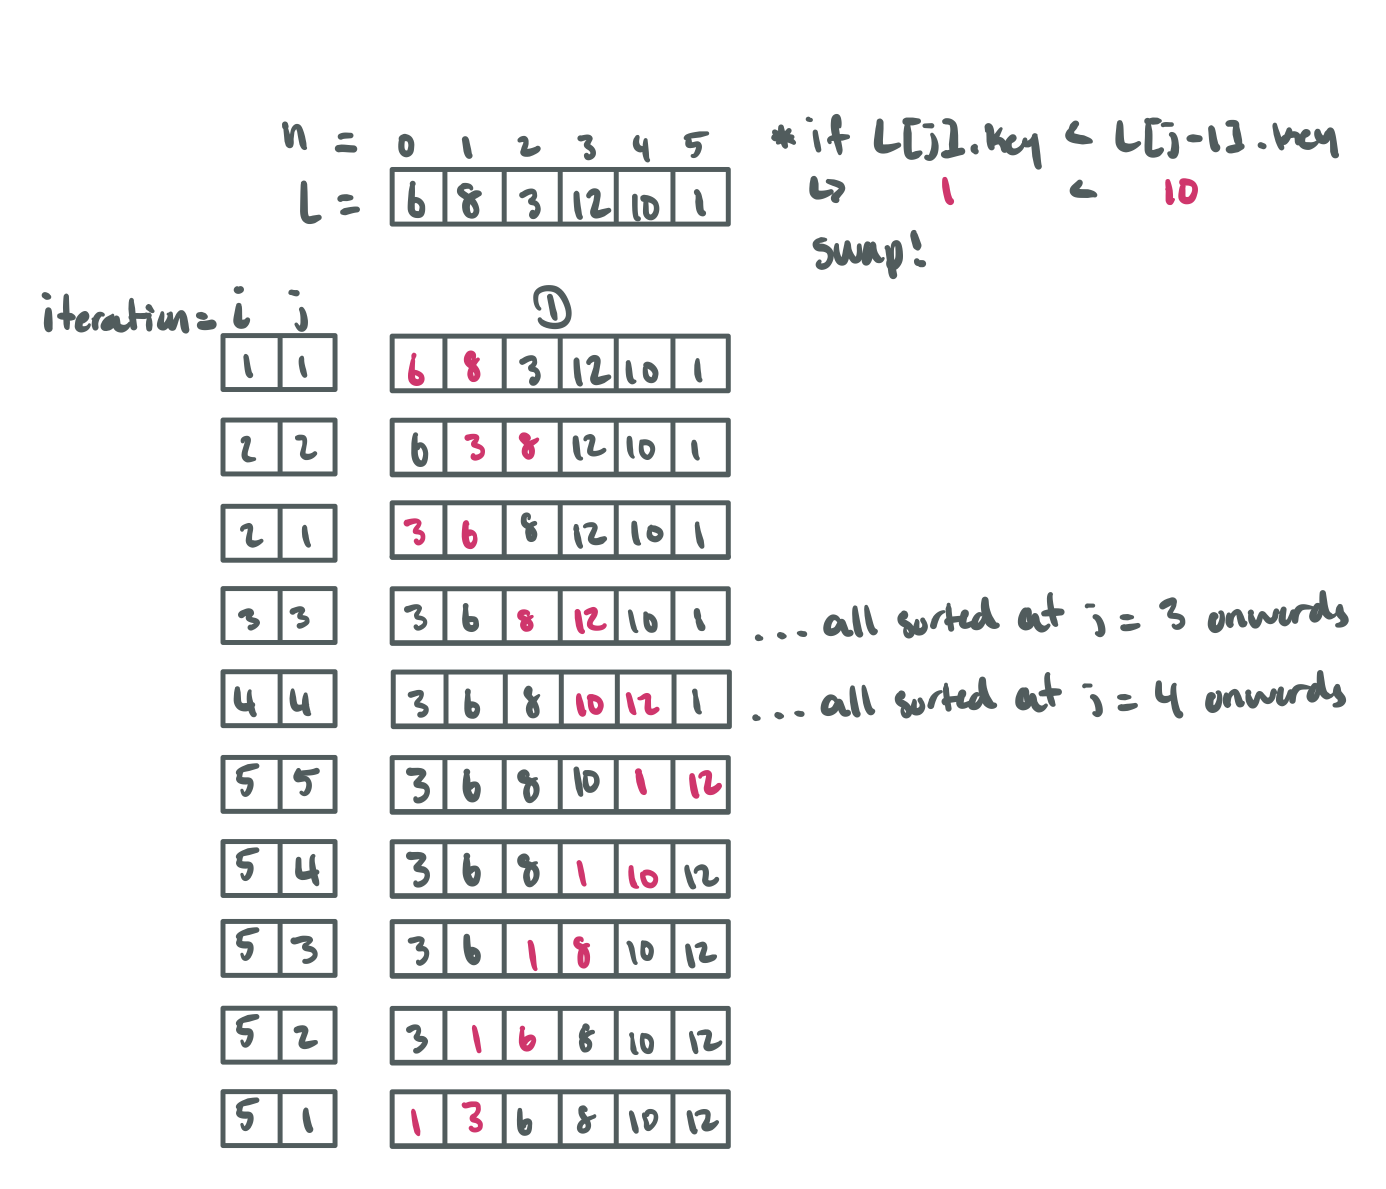
\includegraphics[width=0.76\textwidth]{InsertionSort.png}
        \caption{Insertion sort following the main algorithm}
    \end{center}
\end{figure}

%----Time Complexity----%
\begin{definition}
    \textit{Time Complexity}
    \begin{itemize}
        \item \textbf{swap()}: $\theta(1)$
        \item \textbf{j-loop}: executed $i$ times
        \item \textbf{i-loop}: executed $n-1$ times, $\theta(n)$
        \item \textbf{Insertion-Sort}: $\Sigma^{n-1}_{i=1}n-i-1$ $$\Sigma^{n-1}_{i=1}n-i-1=(n-1)+(n-2)+...+1+0=\frac{n^2-n}{2}$$
        \item \textbf{Hence}, Insertion-Sort is quadratic, $\theta(n^2)$
    \end{itemize}
\end{definition}

%----Correctness----%
\subsubsection{Correctness}
\begin{definition}
    \textit{Loop Invariant}
    \begin{itemize}
        \item \textbf{Inner Loop}
        \begin{itemize}
            \item \textit{\textbf{Initialization}}:
            \begin{itemize}
                \item Initially, $j=i=1$, $L[0...0]$ is a sorted permutation of $S[0]$
                \begin{itemize}
                    \item LI is vacuously satsified
                \end{itemize}
            \end{itemize}
            \item \textit{\textbf{Maintenance}}:
            \begin{itemize}
                \item Assume LI is correct before iteration $j=k$
                \item Hence, $L[k-1...i-1]$ is a sorted permutation of $S[k-1...i-1]$
                \item We show LI still holds at the end of this iteration before $j=k-1$
                \begin{itemize}
                    \item Loop compares $L[k-1],L[k-2]$
                    \item If $L[k-2].key<L[k-1].key$, swap($L[k-2].key, L[k-1].key$)
                    \item Now, $L[k-2...i-1]$ is also a sorted permutation of $S[k-2...i-1]$
                    \item Else, $L[k-2].key$ is larger than $L[k-1].key$, loop does nothing and $L[k-2...i-1]$ is still a sorted
                    permutation of $S[k-2...i-1]$
                \end{itemize}
                \item In both cases, the loop makes sure $L[k-2...i-1]$ has the same items as $S[k-2...i-1]$
                \item Hence, LI still holds at the end of the iteration
            \end{itemize}
            \item \textit{\textbf{Termination}}:
            \begin{itemize}
                \item Last iteration of the loop is when $j=1$
                \item Always terminates because $j$ will eventually reach 0, which is the condition for the for-loop to be false
                \item Hence, at the end of it, $L[0...i-1]$ is a sorted permutation of $S[0...i-1]$ where $i\in[1,n]$
            \end{itemize}
        \end{itemize}
        \item \textbf{Outer Loop}
        \begin{itemize}
            \item \textit{\textbf{Initialization}}:
            \begin{itemize}
                \item Before the first iteration, $i=1$ and $L[1...n-1]$ is empty and LI is vacuously true
            \end{itemize}
            \item \textit{\textbf{Maintenance}}:
            \begin{itemize}
                \item Assume LI is correct before iteration $i=k$
                \item Hence, by the inner LI, $L[0...n-2]$ is a sorted permutation of $S[0...n-2]$ after the last iteration of the outer loop
                \item Suffices to note that when $i=n-1$ (last iteration of the outer loop)
                \item If $L[n-2].key < L[n-1].key$, swap
                \item Else, don't do anything
                \item Hence, $L[0...n-1]$ is a sorting of $S[0...n-1]$
            \end{itemize}
            \item \textit{\textbf{Termination}}:
            \begin{itemize}
                \item Last iteration of the loop is when $i=n-1$
                \item Starts with $i=1$
                \item $i$ doesn't change anywhere other than incrementation
                \item $i$ will eventually become $n$
                \item Hence, Insert-Sort() always terminates
            \end{itemize}
        \end{itemize}
    \end{itemize}
\end{definition}
\newpage
%-----------------------------------------------------------------------------------%
%--Heap Sort--%
\subsection{Heap Sort}
%----Algorithm----%
%----Time Complexity----%
%----Correctness----%
\newpage
%-----------------------------------------------------------------------------------%
%Advanced Sorting Algorithms
\section{Advanced Sorting Algorithms}
%--Merge Sort--%
\subsection{Merge Sort}
%----Algorithm----%
%----Time Complexity----%
%----Correctness----%
\newpage
%-----------------------------------------------------------------------------------%
%--Quick Sort--%
\subsection{Quick Sort}
%----Algorithm----%
%----Time Complexity----%
%----Correctness----%
\newpage
%-----------------------------------------------------------------------------------%

%Searching%
\section{Searching}
%--Linear Search--%
\subsection{Linear Search}
%----Algorithm----%
%----Time Complexity----%
%----Correctness----%
\newpage
%-----------------------------------------------------------------------------------%
%--Binary Search--%
\subsection{Binary Search}
%----Algorithm----%
%----Time Complexity----%
%----Correctness----%
\newpage
%-----------------------------------------------------------------------------------%

%Graph Traversal%
\section{Graph Traversal}
%--Depth-first Search--%
\subsection{Depth-First Search}
%----Algorithm----%
%----Time Complexity----%
%----Correctness----%
%----Applications----%
\newpage
%-----------------------------------------------------------------------------------%
%--Breadth-first Search--%
\subsection{Breadth-First Search}
%----Algorithm----%
%----Time Complexity----%
%----Correctness----%
%----Applications----%
\newpage
%-----------------------------------------------------------------------------------%

\end{document}
